%%%%%%%%%%%%%%%%%%%%%%%%%%%%%%%%%%%%%%%%%
% DeepEarth WMW 2026 Poster
%%%%%%%%%%%%%%%%%%%%%%%%%%%%%%%%%%%%%%%%%

\documentclass[25pt, a0paper, portrait]{tikzposter}

\usepackage{graphicx}
\usepackage{amsmath}
\usepackage{amssymb}
\usepackage{bm}
\usepackage{booktabs}
\usepackage{url}
\usepackage{xcolor}
\usepackage[hidelinks]{hyperref}
\usepackage{enumitem}
\usepackage{fontspec}
\usepackage{tcolorbox}

% GitHub Dark exact colors from github.com (softer background)
\definecolor{ghbg}{HTML}{24292e}        % Softer dark gray background
\definecolor{ghtext}{HTML}{c9d1d9}      % Default text
\definecolor{ghkeyword}{HTML}{ff7b72}   % Keywords (from, import, if, else)
\definecolor{ghstring}{HTML}{a5d6ff}    % Strings
\definecolor{ghcomment}{HTML}{8b949e}   % Comments
\definecolor{ghnumber}{HTML}{79c0ff}    % Numbers
\definecolor{ghfunction}{HTML}{d2a8ff}  % Function/class names
\definecolor{ghconstant}{HTML}{79c0ff}  % Constants (True, False)

% Monospace font for code (Menlo - similar to GitHub's SF Mono)
\newfontfamily\ghcodefont{Menlo}[Scale=0.9]

% Oxygen font family (ligatures disabled to fix Ghostscript compression issues)
\setmainfont{Oxygen}[
    Path = /Users/lancelegel/Library/Fonts/,
    Extension = .ttf,
    UprightFont = *-Regular,
    BoldFont = *-Bold,
    Ligatures = {NoRequired, NoCommon, NoContextual},
    ItalicFont = *-Regular,
    BoldItalicFont = *-Bold,
]
\newfontfamily\oxygenlight{Oxygen-Light}[
    Path = /Users/lancelegel/Library/Fonts/,
    Extension = .ttf,
    Ligatures = {NoRequired, NoCommon, NoContextual}
]
\newfontfamily\oxygenbold{Oxygen-Bold}[
    Path = /Users/lancelegel/Library/Fonts/,
    Extension = .ttf,
    Ligatures = {NoRequired, NoCommon, NoContextual}
]

\graphicspath{{../figures/}{logos/}{renders/}{./}}

% Theme color from header
\definecolor{themeblue}{HTML}{164e72}

\definecolorstyle{DeepEarthStyle}{
    \definecolor{colorOne}{HTML}{164e72}
    \definecolor{colorTwo}{HTML}{164e72}
    \definecolor{colorThree}{HTML}{f0f5f8}
}{
    \colorlet{backgroundcolor}{white}
    \colorlet{framecolor}{colorOne}
    \colorlet{titlefgcolor}{themeblue}
    \colorlet{titlebgcolor}{white}
    \colorlet{blocktitlebgcolor}{colorOne}
    \colorlet{blocktitlefgcolor}{white}
    \colorlet{blockbodybgcolor}{white}
    \colorlet{blockbodyfgcolor}{black}
    \colorlet{innerblocktitlebgcolor}{colorThree}
    \colorlet{innerblocktitlefgcolor}{black}
    \colorlet{innerblockbodybgcolor}{colorThree}
    \colorlet{innerblockbodyfgcolor}{black}
    \colorlet{notefgcolor}{black}
    \colorlet{notebgcolor}{colorThree}
    \colorlet{noteframecolor}{colorOne}
}

\defineblockstyle{CleanBlock}{
    titlewidthscale=1, bodywidthscale=1, titleleft,
    titleoffsetx=0pt, titleoffsety=0pt, bodyoffsetx=0pt, bodyoffsety=0pt,
    bodyverticalshift=0pt, roundedcorners=10, linewidth=1.5pt,
    titleinnersep=6mm, bodyinnersep=6mm
}{
    \begin{scope}[line width=\blocklinewidth, rounded corners=\blockroundedcorners]
        \ifBlockHasTitle
            \draw[fill=blocktitlebgcolor, draw=none]
                (blocktitle.south west) rectangle (blocktitle.north east);
            \draw[fill=blockbodybgcolor, draw=framecolor]
                (blockbody.south west) rectangle (blockbody.north east);
        \else
            \draw[fill=blockbodybgcolor, draw=framecolor]
                (blockbody.south west) rectangle (blockbody.north east);
        \fi
    \end{scope}
}

\definetitlestyle{MinimalTitle}{
    width=\paperwidth, roundedcorners=0, linewidth=0pt, innersep=0mm,
    titletotopverticalspace=0mm, titletoblockverticalspace=6mm
}{
}

\usetheme{Default}
\usecolorstyle{DeepEarthStyle}
\usetitlestyle{MinimalTitle}
\useblockstyle{CleanBlock}

\tikzposterlatexaffectionproofoff

\setlist[itemize]{noitemsep, topsep=2pt, leftmargin=12pt, parsep=0pt, itemsep=2pt}
\setlist[enumerate]{noitemsep, topsep=2pt, leftmargin=12pt, parsep=0pt, itemsep=2pt}

\title{}
\author{}
\institute{}

\begin{document}

\maketitle

% Header from user's PDF
\block{}{
\vspace{-2mm}
\centering
\includegraphics[width=\linewidth]{wmw2026_poster_header.pdf}
\vspace{-2mm}
}

\begin{columns}

\column{0.5}

%-----------------------------------------------------------------------
\block{DeepEarth Architecture}{
\vspace{1mm}
\centering
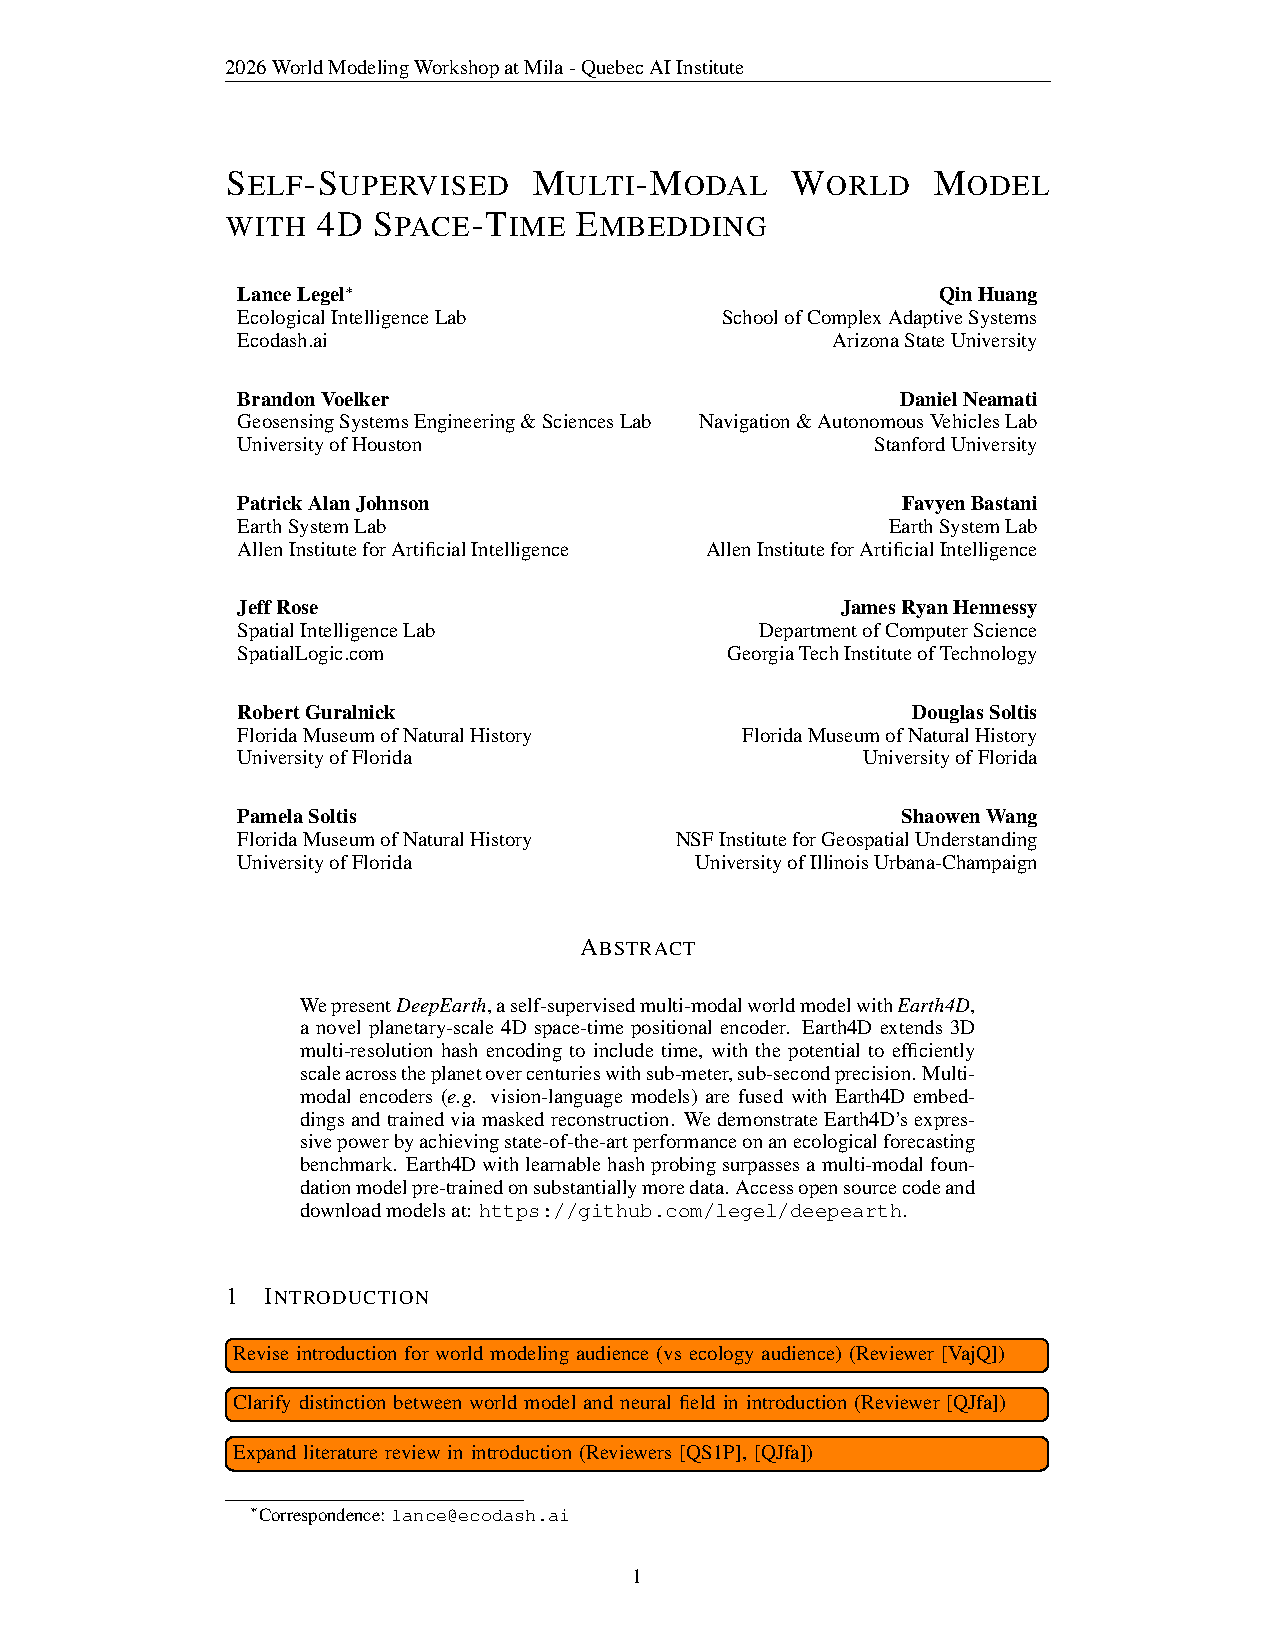
\includegraphics[width=\linewidth]{deepearth.pdf}

\vspace{3mm}
\raggedright
{\normalsize\oxygenbold Figure 1.} {\normalsize\oxygenlight Self-supervised multi-modal world model for planetary science, simulation, \& planning.}

\vspace{4mm}
\begin{itemize}
\item {\oxygenbold Earth4D} encodes $(x,y,z,t)$ coordinates into learnable space-time embeddings
\item Fuses multi-modal ($e.g.$ vision-language) and space-time embeddings
\item Trains by masked reconstruction of multi-modal data across space-time
\end{itemize}
\vspace{1mm}
}

%-----------------------------------------------------------------------
\block{Key Contributions}{
\vspace{1mm}
\begin{enumerate}[leftmargin=*, labelsep=3mm]
\item {\oxygenbold Space-Time Positional Encoder:} Unify all kinds of physical data modalities
\item {\oxygenbold Multi-Scale 4D Geospatial Simulator:} Bridge planetary-to-cellular dynamics
\item {\oxygenbold 4D Learned Hash Probing:} Dif{}ferentiably map ($x$,$y$,$z$,$t$) $\rightarrow$ embedding indices
\end{enumerate}

\vspace{1mm}
}

%-----------------------------------------------------------------------
\block{State-of-the-Art Ecological Prediction Benchmark}{
\vspace{1mm}
Live Fuel Moisture Content (LFMC) measures vegetation water for wildf{}ire risk.\\
{\oxygenbold Training:} Earth4D encodes ($x$, $y$, $z$, $t$) coordinates of LFMC metrics to 192D, concatenates with learnable plant species embeddings, MLP predicts LFMC.\\
{\oxygenbold Result:} Earth4D outperforms pre-trained Vision Transformer with less input data.

\vspace{4mm}
\centering
\includegraphics[width=\linewidth]{error_distribution_histogram.png}

\vspace{2mm}
\includegraphics[width=\linewidth]{geospatial_temporal_test.png}

\vspace{3mm}
\raggedright
{\normalsize\oxygenbold Figure 4.} {\normalsize\oxygenlight Earth4D LFMC test predictions on Allen Institute for AI (AI2) Globe-LFMC 2.0 benchmark.}

\vspace{14mm}
\centering
{\fontsize{28}{33}\selectfont
\begin{tabular}{@{}l l c c c@{}}
\toprule
{\oxygenbold Model} & {\oxygenbold Data Inputs} & {\oxygenbold MAE} & {\oxygenbold RMSE} & {\oxygenbold R²} \\
\midrule
AI2 (Pre-trained ViT) & ($x$,$y$,$z$,$t$) + Species + Vision (Remote Sensing) & 12.6pp & 18.9pp & 0.72 \\
{\oxygenbold Earth4D} & ($x$,$y$,$z$,$t$) + Species & {\oxygenbold 11.7pp} & {\oxygenbold 18.7pp} & {\oxygenbold 0.783} \\
\bottomrule
\end{tabular}
}

\vspace{10mm}
\raggedright
{\oxygenbold Key Finding:} Earth4D surpasses AI2's foundation model without satellite, weather, or topography data. Only coordinates and species names are used.
\vspace{1mm}
}

%-----------------------------------------------------------------------

\column{0.5}

%-----------------------------------------------------------------------
\block{Earth4D Space-Time Positional Encoding}{
\vspace{1mm}
\centering
\includegraphics[width=\linewidth]{earth4d.pdf}

\vspace{3mm}
\raggedright
{\normalsize\oxygenbold Figure 2.} {\normalsize\oxygenlight Multi-resolution hash encoding extended to 4D space-time across the planet over years.}

\vspace{4mm}
Earth4D: {\oxygenbold multi-resolution hash encoder} with four parallel 3D grids.\\
{\oxygenbold Spatial} ($xyz$): static structure. {\oxygenbold Spatio-temporal} ($xyt$, $yzt$, $xzt$): dynamics.

\vspace{3mm}
{\oxygenbold Geographic:} Maps ($latitude$, $longitude$, $elevation$, $time$) $\rightarrow$ ($x$, $y$, $z$, $t$)
\vspace{1mm}
}

%-----------------------------------------------------------------------
\block{Joint Embeddings Across Spatio-Temporal Scales}{
\vspace{1mm}
\centering
\includegraphics[width=\linewidth]{earth4d_resolution_levels.png}

\vspace{3mm}
{\normalsize\oxygenbold Figure 3.} {\normalsize\oxygenlight 24 resolution levels per grid ($xyz$, $xyt$, $yzt$, $xzt$), up to $2^{22}$ entries each.}\\
{\normalsize\oxygenlight Output: 192D trainable embedding per ($x$,$y$,$z$,$t$) coordinate.}
\vspace{1mm}
}

%-----------------------------------------------------------------------
\block{Learned Hash Probing}{
\vspace{1mm}
Hash encoding compresses features into f{}ixed memory, but collisions hurt accuracy. {\oxygenbold Learned hash probing} optimizes memory allocation end-to-end.

\vspace{3mm}
{\oxygenbold Performance:} 33\% fewer collisions; MAE improved 27\%; R² improved 30\%.
\vspace{1mm}
}

%-----------------------------------------------------------------------
\block{Code Demo: Space-Time Positional Encoding}{
\vspace{-2mm}
\begin{tcolorbox}[
    colback=ghbg,
    colframe=ghbg,
    boxrule=0pt,
    arc=6pt,
    left=12pt,
    right=12pt,
    top=6pt,
    bottom=6pt,
    width=\linewidth
]
\ghcodefont\fontsize{26}{33}\selectfont\color{ghtext}
\noindent{\color{ghcomment}\# https://github.com/legel/deepearth}\\[5pt]
{\color{ghkeyword}from} deepearth.encoders.xyzt.earth4d {\color{ghkeyword}import} {\color{ghfunction}Earth4D}\\[5pt]
world\_model = {\color{ghfunction}Earth4D}()\\[5pt]
embeddings = {\color{ghfunction}world\_model}(\\[2pt]
\hspace*{24pt}{\color{ghcomment}\# Bletchley Park (Turing breaks Enigma, 1941)}\\[2pt]
\hspace*{24pt}({\color{ghnumber}51.9976}, {\color{ghnumber}-0.7416}, {\color{ghnumber}110}, {\color{ghstring}"1941-06-01 09:00 GMT"}),\\[2pt]
\hspace*{24pt}{\color{ghcomment}\# Carnegie Mellon (Hinton invents Boltzmann Machines, 1985)}\\[2pt]
\hspace*{24pt}({\color{ghnumber}40.4433}, {\color{ghnumber}-79.9436}, {\color{ghnumber}270}, {\color{ghstring}"1985-01-15 10:00 ET"}),\\[2pt]
\hspace*{24pt}{\color{ghcomment}\# CERN (Berners-Lee invents WWW, 1989)}\\[2pt]
\hspace*{24pt}({\color{ghnumber}46.2330}, {\color{ghnumber}6.0557}, {\color{ghnumber}430}, {\color{ghstring}"1989-03-12 10:00 CET"}),\\[2pt]
\hspace*{24pt}{\color{ghcomment}\# Mila, Quebec (World Modeling Workshop 2026)}\\[2pt]
\hspace*{24pt}({\color{ghnumber}45.5308}, {\color{ghnumber}-73.6128}, {\color{ghnumber}63}, {\color{ghstring}"2026-02-04 11:00 ET"}),\\[2pt]
)\\[5pt]
{\color{ghcomment}\# embeddings.shape: [4, 192] -- trainable space-time features}
\end{tcolorbox}
\vspace{-2mm}
}

%-----------------------------------------------------------------------
\block{References}{
\vspace{1mm}
{\fontsize{19}{23}\selectfont
\begin{enumerate}
\item Müller et al. {\oxygenbold ``Instant Neural Graphics Primitives with a Multiresolution Hash Encoding.''} {\itshape ACM SIGGRAPH}, 2022.
\item Takikawa et al. {\oxygenbold ``Compact Neural Graphics Primitives with Learned Hash Probing.''} {\itshape SIGGRAPH Asia}, 2023.
\item Xu et al. {\oxygenbold ``Grid4D: 4D Decomposed Hash Encoding for High-f{}idelity Dynamic Gaussians.''} {\itshape NeurIPS}, 2024.
\item Yebra et al. {\oxygenbold ``Globe-LFMC 2.0: Enhanced global dataset for live fuel moisture.''} {\itshape Scientif{}ic Data}, 2024.
\item Tseng et al. {\oxygenbold ``Galileo: Learning Global and Local Features of Many Remote Sensing Modalities.''} {\itshape ICML}, 2025.
\item Johnson et al. {\oxygenbold ``High-Resolution LFMC Maps for Wildf{}ire Risk From Multimodal Earth Observation Data.''} {\itshape PMLR}, 2025.
\end{enumerate}
}
\vspace{1mm}
}

\end{columns}

\vspace{4mm}
\centering
{\Large\textbf{2026 World Modeling Workshop at Mila, Quebec AI Institute}}

\end{document}
